\documentclass[12pt,a4paper]{ctexart}

% 基础宏包
\usepackage{amsmath,amssymb,amsfonts}
\usepackage{graphicx}
\usepackage{booktabs}
\usepackage{multirow}
\usepackage{enumitem}
\usepackage{hyperref}
\usepackage{url}
\usepackage{caption}
\usepackage{subcaption}
\usepackage{float}
\usepackage{geometry}
\usepackage[numbers,sort&compress]{natbib}

% 页面设置
\geometry{left=2.5cm, right=2.5cm, top=2.5cm, bottom=2.5cm}

% 超链接设置
\hypersetup{
  colorlinks=true,
  linkcolor=blue,
  citecolor=blue,
  urlcolor=blue,
  bookmarks=true
}

% 图表标题设置
\captionsetup{font=small, labelsep=space}
\renewcommand{\figurename}{图}
\renewcommand{\tablename}{表}

% 数学符号
\newcommand{\R}{\mathbb{R}}
\newcommand{\E}{\mathbb{E}}
\DeclareMathOperator*{\argmin}{arg\,min}
\DeclareMathOperator*{\argmax}{arg\,max}

% 作者信息（请替换为真实姓名和学号）
\title{\textbf{基于OpenPCDet的三维点云目标检测对抗攻击与安全性验证}}

\author{
  张三\textsuperscript{1} \quad 李四\textsuperscript{1} \quad 王五\textsuperscript{1} \quad 赵六\textsuperscript{1} \quad 钱七\textsuperscript{1}
}

\date{
  \small\textsuperscript{1} XX大学 计算机科学与技术学院, XX 省 XX 市 XXXXXX\\[2pt]
  \small Email: \{zhangsan, lisi, wangwu, zhaoliu, qianqi\}@xxx.edu.cn
}

\begin{document}
\maketitle

\vspace{-1em}
\noindent\rule{\textwidth}{0.4pt}

% ============================================================
% 摘要
% ============================================================
\begin{abstract}
随着自动驾驶技术的快速发展，基于LiDAR点云的三维目标检测已成为感知系统的核心模块。然而，深度神经网络对对抗样本的脆弱性引发了严重的安全隐患。本文基于OpenPCDet工业级检测框架和PointPillars模型，系统化实现了针对三维点云目标检测的对抗攻击与安全性评估。我们设计了双通道攻击注入架构，实现6类10种攻击算法（包括坐标微扰、随机删除、几何感知删除、梯度扰动、显著性掩码删除及对抗点/物体插入），并在KITTI验证集（3769个样本）上完成全量mAP评估。实验结果表明：(1)~高斯噪声攻击在强度$\sigma \geq 0.3$时即可导致检测器完全崩溃（Car AP从78.40降至6.90）；(2)~几何感知删除比随机删除更有效（AP下降55\% vs 11\%@severity=0.5）；(3)~白盒梯度攻击可将AP降至接近零；(4)~插入类攻击对AP影响极小，因其攻击机制与AP评价指标存在不匹配。本研究为三维点云感知系统的安全性评估提供了系统化的攻击基准和实验依据。
\end{abstract}

\noindent\textbf{关键词：}三维点云；对抗攻击；目标检测；PointPillars；安全性验证；OpenPCDet

% ============================================================
% 1 引言
% ============================================================
\section{引言}

自动驾驶技术的安全可靠性是当前学术界和工业界共同关注的核心问题。LiDAR（激光雷达）传感器通过发射激光脉冲获取环境的三维点云数据，为自动驾驶车辆提供了精确的空间感知能力。基于深度学习的三维目标检测模型（如PointPillars\cite{lang2019pointpillars}、SECOND\cite{yan2018second}）已在KITTI基准\cite{geiger2012kitti}上取得了优异的性能，但这些模型对对抗样本的鲁棒性仍是一个亟待研究的问题。

对抗攻击的研究起源于二维图像领域。Szegedy等人\cite{szegedy2014intriguing}首次发现深度神经网络对精心构造的微小扰动极为敏感，Goodfellow等人\cite{goodfellow2015explaining}随后提出了快速梯度符号方法（FGSM），将对抗攻击形式化为一个优化问题。Carlini和Wagner\cite{carlini2017towards}进一步提出了C\&W攻击，Madry等人\cite{madry2018towards}则提出了投影梯度下降（PGD）攻击，这些工作共同建立了二维对抗攻击的理论基础。

将对抗攻击从二维图像扩展到三维点云面临新的挑战。点云数据具有无序性、稀疏性和三维几何结构等特性，使得传统的图像对抗方法不能直接迁移。Xiang等人\cite{xiang2019generating}在CVPR 2019上提出了针对点云分类模型的三种对抗攻击方法——坐标微扰（Perturbation）、关键点删除（Dropping）和对抗点生成（Generation），为三维点云对抗攻击奠定了理论基础。然而，该工作仅针对PointNet/PointNet++分类任务，尚未在工业级目标检测框架上得到验证。

Zhang等人\cite{zhang2023robust3dod}在Robust3DOD工作中对LiDAR三维目标检测器的鲁棒性进行了综合研究，但该工作需要对检测框架进行较大修改（删除\texttt{@torch.no\_grad()}装饰器以启用梯度回传），且未完全解决OpenPCDet中5个梯度断裂点的端到端传播问题。

\textbf{本文的主要贡献如下：}
\begin{enumerate}[label=(\arabic*)]
  \item 在OpenPCDet工业级框架\cite{openpcdet2020}上设计了双通道攻击注入架构，实现6类10种攻击算法，涵盖扰动、删除、插入三种攻击范式；
  \item 在KITTI验证集（3769个样本）上完成全量$\text{AP}_{R40}$评估，建立了黑盒攻击与白盒攻击的系统化对比基准；
  \item 提出几何感知删除攻击（geo\_drop），通过优先删除距点云质心最近的点来破坏目标几何特征，实验证明其效果显著优于随机删除；
  \item 对攻击效果进行了多维度分析，揭示了不同攻击类型、强度等级和目标类别之间的关系。
\end{enumerate}

本文的完整代码、实验数据和可视化结果已开源于GitHub\footnote{\url{https://github.com/twolate0101/OpenPCDet-Adversarial-Attack}}，欢迎复现和验证。

% ============================================================
% 2 相关工作
% ============================================================
\section{相关工作}

\subsection{三维点云目标检测}

三维点云目标检测旨在从LiDAR采集的点云数据中定位和分类三维目标。PointNet\cite{qi2017pointnet}和PointNet++\cite{qi2017pointnetplusplus}开创性地将深度学习直接应用于无序点集，通过对称函数实现置换不变性。PointPillars\cite{lang2019pointpillars}提出将三维点云编码为伪图像（Pillar体素化），使得成熟的二维卷积网络可直接复用，在KITTI基准上取得了实时性和精度的良好平衡。SECOND\cite{yan2018second}引入稀疏卷积，高效处理三维空间的稀疏性。本文选择PointPillars作为目标检测模型，KITTI验证集作为评估基准。

\subsection{对抗攻击理论基础}

对抗样本的形式化定义如下。给定训练好的分类器$f$和干净输入$x$，对抗样本$x_{\text{adv}}$满足：
\begin{equation}
  f(x_{\text{adv}}) \neq f(x), \quad \text{s.t.} \quad \|x_{\text{adv}} - x\|_p \leq \epsilon
  \label{eq:adv_def}
\end{equation}
其中$\epsilon$控制扰动的$L_p$范数预算。

\textbf{FGSM}（Fast Gradient Sign Method）\cite{goodfellow2015explaining}利用损失函数关于输入的梯度方向生成单步扰动：
\begin{equation}
  x_{\text{adv}} = x + \epsilon \cdot \text{sign}(\nabla_x \mathcal{L}(f(x), y))
  \label{eq:fgsm}
\end{equation}

\textbf{PGD}（Projected Gradient Descent）\cite{madry2018towards}是FGSM的多步迭代版本，每步后投影回$\epsilon$球约束内：
\begin{equation}
  x_{t+1} = \Pi_{\mathcal{B}_\epsilon(x)}\left(x_t + \alpha \cdot \text{sign}(\nabla_x \mathcal{L}(f(x_t), y))\right)
  \label{eq:pgd}
\end{equation}
其中$\alpha$为步长，$\Pi_{\mathcal{B}_\epsilon(x)}$为投影算子。

\textbf{C\&W攻击}\cite{carlini2017towards}将对抗样本生成建模为约束优化问题：
\begin{equation}
  \min_{\delta} \|\delta\|_2^2 + \lambda \cdot f(x + \delta), \quad \text{s.t.} \quad f(x + \delta) \neq y
  \label{eq:cw}
\end{equation}
其中$f(\cdot)$为衡量分类器置信度的损失函数。

\subsection{三维点云对抗攻击的特殊挑战}

将上述二维对抗方法迁移到三维点云目标检测面临独特的挑战。在OpenPCDet框架中，推理链路存在5个梯度断裂点：(1)~体素化过程返回NumPy数组；(2)~稀疏张量索引为整数坐标，不可微；(3)~PillarVFE的max pooling仅最大点获梯度；(4)~BEV Pooling CUDA算子显式标记不可微；(5)~NMS后处理为离散索引选择。这些断裂点使得端到端梯度回传无法实现，PGD和C\&W等白盒攻击方法需要特殊适配。

\section{攻击方法实现}

\subsection{双通道攻击注入架构}

我们设计了双通道攻击注入架构，支持在OpenPCDet推理链路的不同位置注入攻击：

\textbf{通道一（黑盒通道）}：在体素化之前拦截原始点云。攻击器修改$\text{points} \in \R^{N \times 4}$（$N$为点数，4维为$x,y,z,\text{intensity}$），修改后的点云再经过正常的体素化和推理流程。适用于不需要模型梯度的攻击。

\textbf{通道二（白盒通道）}：在体素化之后、模型推理之前，通过\texttt{forward\_pre\_hook}拦截体素数据。攻击器修改$\text{voxels} \in \R^{M \times P \times 4}$（$M$为体素数，$P$为每体素点数），可利用模型梯度进行优化。

\subsection{黑盒攻击方法}

\subsubsection{高斯坐标微扰（Noise）}

给定原始点云$\mathcal{P} = \{p_i = (x_i, y_i, z_i, r_i)\}_{i=1}^{N}$，噪声攻击为每个点的三维坐标添加独立高斯噪声：
\begin{equation}
  p_i' = p_i + (\delta_x, \delta_y, \delta_z, 0), \quad \delta_x, \delta_y, \delta_z \sim \mathcal{N}(0, \sigma^2)
  \label{eq:noise}
\end{equation}
其中$\sigma = \text{severity}$控制噪声强度。反射率$r_i$保持不变。该攻击模拟LiDAR传感器受干扰或物理微振场景。

\subsubsection{随机点删除（Drop）}

随机删除攻击按severity比例随机丢弃点云中的点：
\begin{equation}
  \mathcal{P}' = \{p_i \mid i \in S\}, \quad |S| = \lfloor(1 - s) \cdot N\rfloor, \quad S \subset \{1,\ldots,N\}
  \label{eq:drop}
\end{equation}
其中$s = \text{severity} \in [0, 1]$为删除比例。保留至少1\%的点以确保体素化不崩溃。该攻击模拟传感器遮挡或信号丢失。

\subsubsection{几何感知删除（Geo-Drop）}

我们提出几何感知删除攻击，其核心思想是优先删除距点云质心最近的点。质心计算为：
\begin{equation}
  \bar{p} = \frac{1}{N}\sum_{i=1}^{N} p_i^{(1:3)}
  \label{eq:centroid}
\end{equation}
计算每个点到质心的欧氏距离：
\begin{equation}
  d_i = \|p_i^{(1:3)} - \bar{p}\|_2
  \label{eq:dist}
\end{equation}
保留距离最远的$K = \lfloor(1-s)\cdot N\rfloor$个点：
\begin{equation}
  \mathcal{P}' = \{p_i \mid d_i \in \text{top-}K \text{ largest}\}
  \label{eq:geodrop}
\end{equation}
由于目标物体通常位于点云密集区域（距质心较近），该策略可更有效地破坏目标的几何特征表达，比随机删除更具针对性。

\subsubsection{幽灵模板注入（Ghost Template）}

在点云空旷区域（$x > 30$m的远处路面）注入预存的目标模板（Car/Pedestrian/Cyclist的长方体表面点云），制造假阳性检测。模板基于真实目标的几何尺寸生成。

\subsection{白盒攻击方法}

\subsubsection{PGD体素扰动（PGD）}

在体素坐标上执行多轮sign-梯度上升，每轮扰动后投影回$L_2$ $\epsilon$球约束内（公式~\ref{eq:pgd}），其中$\epsilon = \text{severity}$，步长$\alpha = \epsilon / T$，$T$为迭代次数。

\subsubsection{C\&W风格体素扰动（Perturb）}

使用Adam优化器迭代调整体素坐标，优化目标为：
\begin{equation}
  \min_{\delta} -\sum_{j} s_j + \lambda \cdot \frac{1}{|\delta|}\|\delta\|_2^2
  \label{eq:perturb}
\end{equation}
其中$s_j$为检测分数，$\lambda$与severity反比：$\lambda = \max(0.5, 1/s)$。

\subsubsection{显著性体素删除（Saliency Mask）}

借鉴JSMA梯度显著性思想，通过一次前向+反向传播获取体素梯度，按梯度绝对值排序后移除对检测贡献最大的Top-$K$\%体素。

\subsubsection{对抗点簇生成（Spawn）与散点放置（Scatter）}

在梯度分析定位的脆弱区域附近，通过Adam优化生成对抗点簇（每簇32点）或独立散点，最小化检测置信度。

\subsubsection{对抗物体放置（Object）}

在脆弱区域放置小型三维立方体（表面32点），联合优化位置偏移、三轴尺寸和旋转角度。

% ============================================================
% 4 实验评估
% ============================================================
\section{实验评估}

\subsection{实验设置}

\textbf{模型}：PointPillars\cite{lang2019pointpillars}，在KITTI训练集上训练7728个epoch，基线性能如表~\ref{tab:baseline}所示。

\textbf{数据集}：KITTI验证集\cite{geiger2012kitti}，包含3769个样本，涵盖城市道路、高速公路等多种驾驶场景。

\textbf{评价指标}：KITTI官方3D AP$_{R40}$（41点插值平均精度），按Car（IoU阈值0.70）、Pedestrian（IoU阈值0.50）、Cyclist（IoU阈值0.50）三个类别分别在Easy、Moderate、Hard三个难度等级上计算。Moderate难度的AP是KITTI排行榜的主指标。

\textbf{攻击参数}：severity $\in \{0.1, 0.3, 0.5\}$，白盒攻击迭代次数$T=20$，batch\_size=4。

\subsection{基线结果}

表~\ref{tab:baseline}展示了PointPillars在无攻击条件下的基线性能。

\begin{table}[H]
\centering
\caption{PointPillars基线性能（3D AP$_{R40}$, KITTI val, 3769样本）}
\label{tab:baseline}
\begin{tabular}{lccc}
\toprule
\textbf{类别} & \textbf{Easy} & \textbf{Moderate} & \textbf{Hard} \\
\midrule
Car (IoU=0.70) & 87.75 & 78.40 & 75.19 \\
Pedestrian (IoU=0.50) & 57.20 & 51.43 & 46.87 \\
Cyclist (IoU=0.50) & 81.56 & 62.92 & 59.03 \\
\bottomrule
\end{tabular}
\end{table}

\subsection{黑盒攻击结果}

表~\ref{tab:blackbox}展示了三种黑盒攻击在不同severity下的全量mAP结果（Moderate难度）。

\begin{table}[H]
\centering
\caption{黑盒攻击全量mAP结果（3D AP$_{R40}$, Moderate难度）}
\label{tab:blackbox}
\begin{tabular}{lccccccccc}
\toprule
\multirow{2}{*}{\textbf{攻击}} & \multicolumn{3}{c}{$s=0.1$} & \multicolumn{3}{c}{$s=0.3$} & \multicolumn{3}{c}{$s=0.5$} \\
\cmidrule(lr){2-4} \cmidrule(lr){5-7} \cmidrule(lr){8-10}
 & Car & Ped & Cyc & Car & Ped & Cyc & Car & Ped & Cyc \\
\midrule
Baseline & 78.40 & 51.43 & 62.92 & 78.40 & 51.43 & 62.92 & 78.40 & 51.43 & 62.92 \\
Noise & 69.85 & 19.56 & 44.02 & 6.90 & 0.01 & 0.07 & 0.00 & 0.00 & 0.00 \\
Drop & 76.36 & 50.31 & 62.87 & 75.62 & 49.39 & 57.91 & 70.04 & 39.89 & 44.60 \\
Geo-Drop & 68.17 & 42.54 & 50.42 & 47.71 & 24.63 & 34.13 & 35.56 & 12.40 & 25.67 \\
\bottomrule
\end{tabular}
\end{table}

图~\ref{fig:map_bar}以分组柱状图直观展示了上述结果。

\begin{figure}[H]
\centering
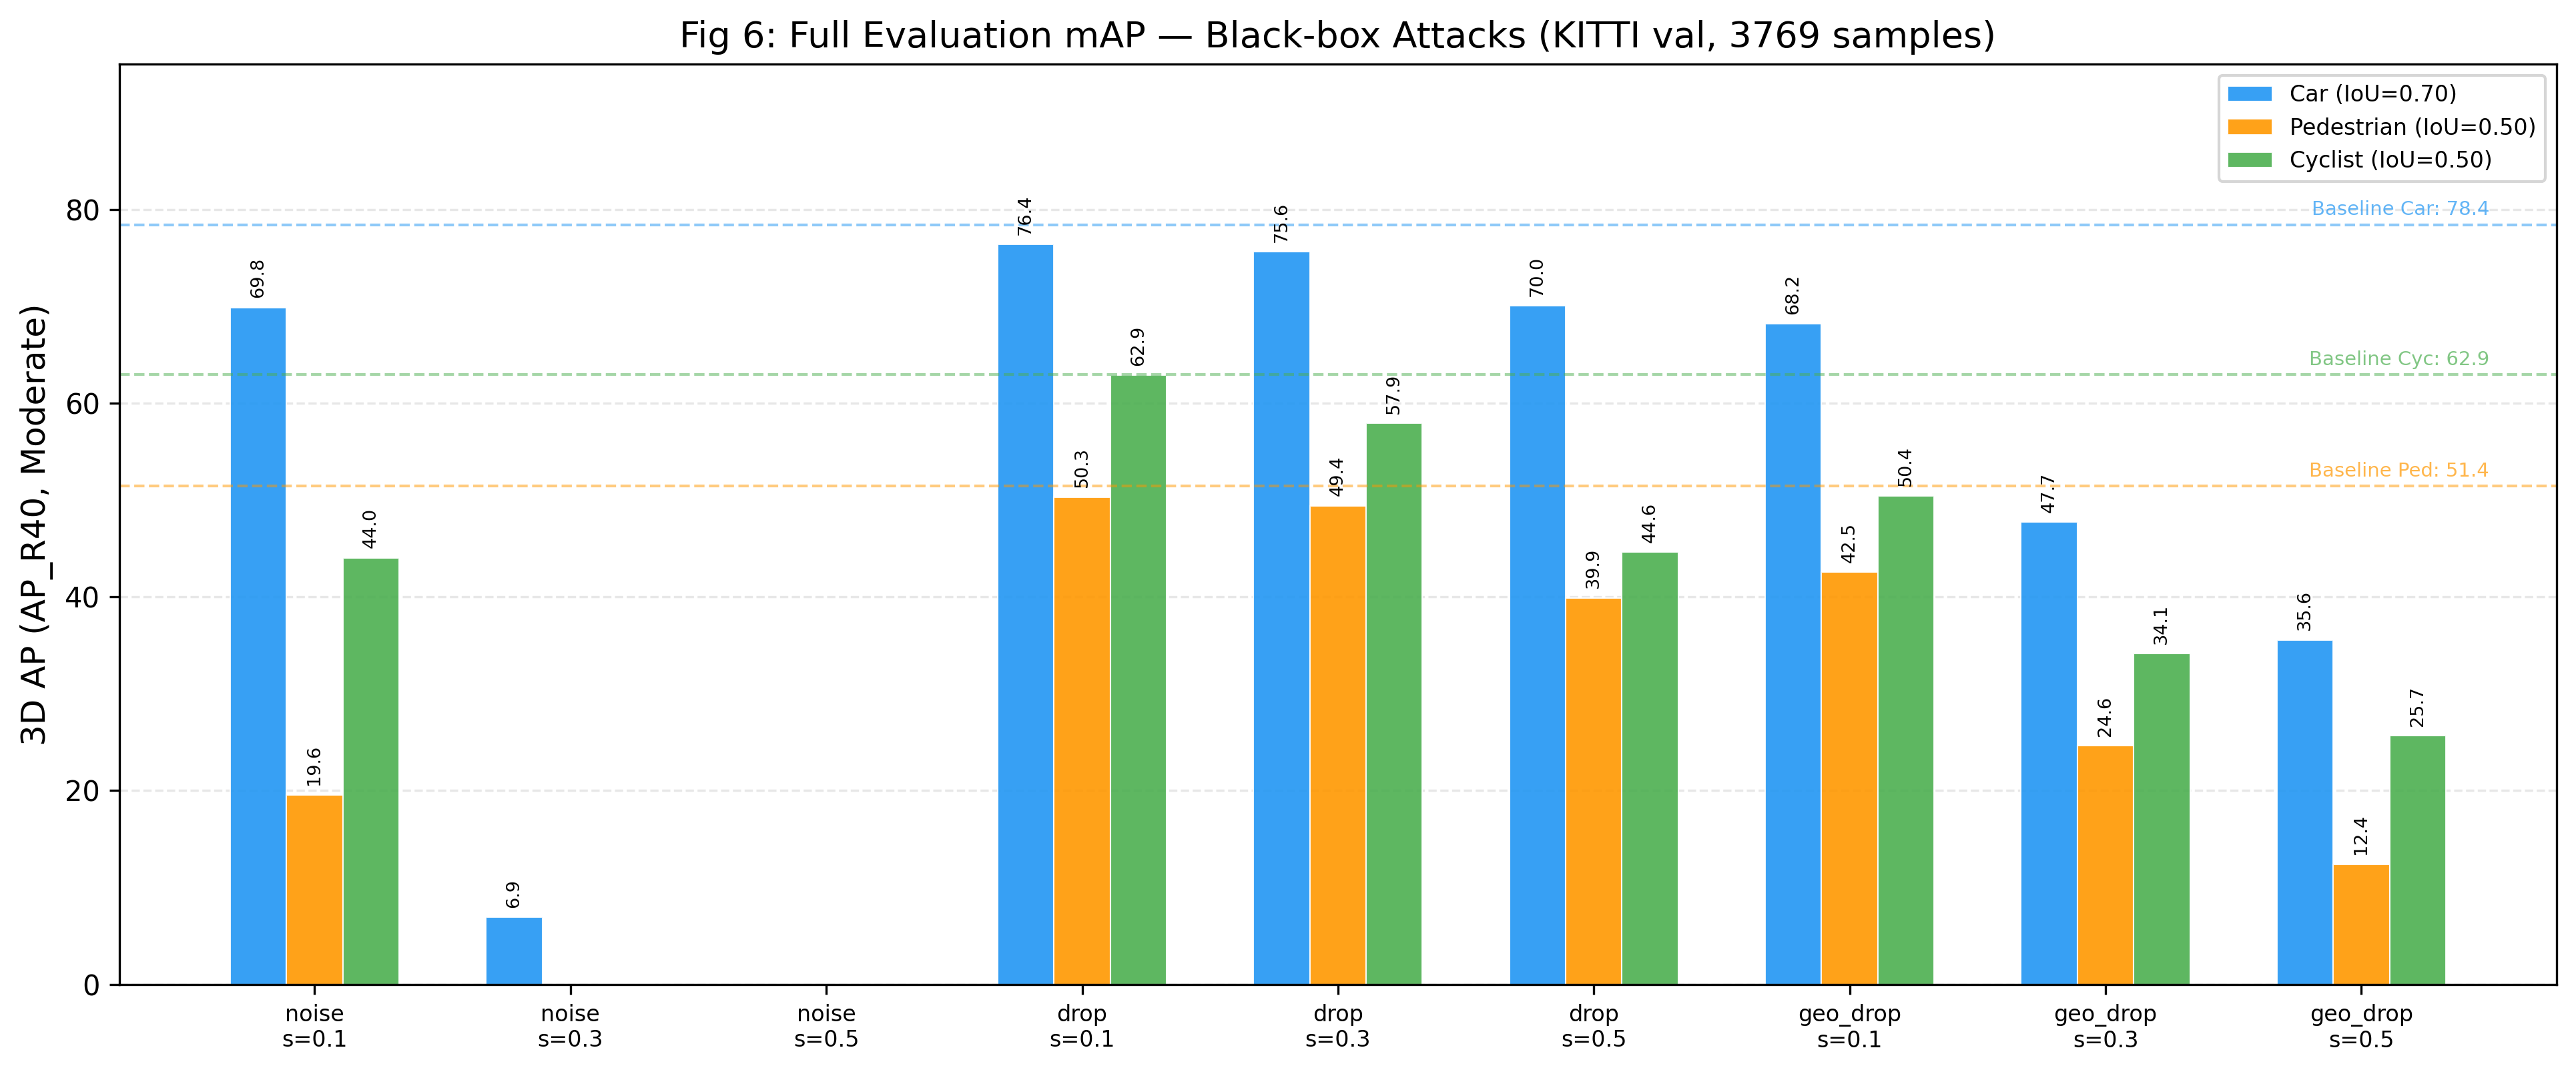
\includegraphics[width=0.95\linewidth]{fig6_map_grouped_bar.png}
\caption{黑盒攻击全量mAP分组柱状图（KITTI val, 3769样本）。虚线为各类别基线。}
\label{fig:map_bar}
\end{figure}

\textbf{关键发现1：噪声攻击的阶跃式崩溃。} 噪声攻击在severity从0.1增加到0.3时呈现阶跃式崩溃——Car AP从69.85骤降至6.90（下降90\%），Pedestrian和Cyclist的AP降至接近零。这表明PointPillars对坐标噪声极其敏感，当噪声标准差$\sigma \geq 0.3$m时，体素化后的几何结构被严重破坏，检测器基本失效。

\textbf{关键发现2：随机删除的温和影响。} 与噪声攻击形成鲜明对比，随机删除即使在severity=0.5时，Car AP仍保持70.04（仅下降11\%）。这是因为点云具有冗余性，随机删除50\%的点后，剩余点仍保留足够的几何信息供检测器推理。

\textbf{关键发现3：几何感知删除的持续有效性。} Geo-Drop的AP下降与severity近似呈线性关系：Car AP从78.40逐步降至68.17（$s=0.1$）、47.71（$s=0.3$）、35.56（$s=0.5$）。相比随机删除，几何感知删除在severity=0.5时多造成34个百分点的AP下降，证明了定向删除策略的优势。

图~\ref{fig:severity}以折线图展示了severity梯度变化趋势。

\begin{figure}[H]
\centering
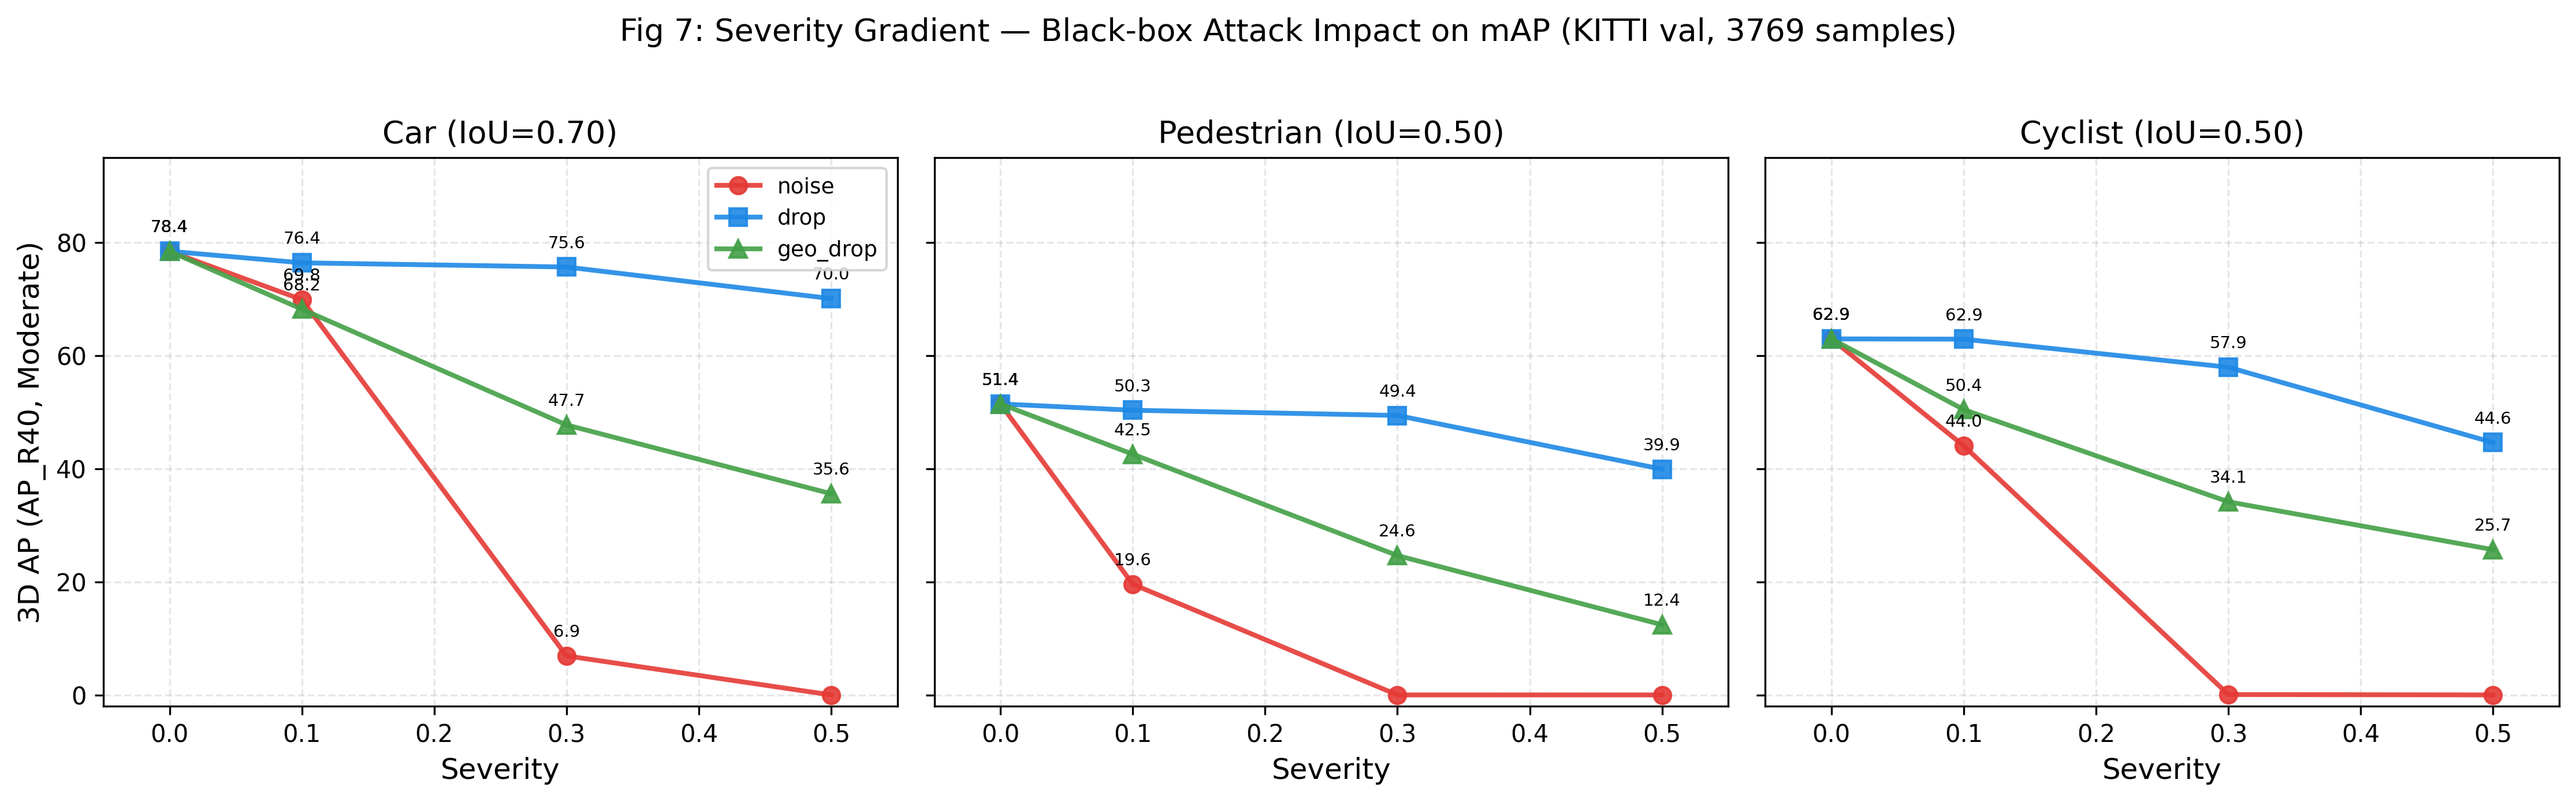
\includegraphics[width=0.95\linewidth]{fig7_severity_curves.png}
\caption{Severity梯度曲线：三类目标在不同攻击下的AP变化趋势。}
\label{fig:severity}
\end{figure}

\subsection{白盒攻击结果}

表~\ref{tab:whitebox}展示了白盒攻击的mAP结果。

\begin{table}[H]
\centering
\caption{白盒攻击mAP结果（3D AP$_{R40}$, Moderate难度, 最佳severity）}
\label{tab:whitebox}
\begin{tabular}{llcccc}
\toprule
\textbf{攻击} & \textbf{类型} & $s$ & \textbf{Car} & \textbf{Ped} & \textbf{Cyc} \\
\midrule
PGD & 白盒扰动 & 0.3 & 0.14 & 0.09 & 0.12 \\
Perturb & 白盒扰动 & 0.5 & 0.60 & 0.78 & 1.39 \\
Saliency Mask & 白盒删除 & 0.3 & 37.06 & 0.00 & 0.02 \\
Spawn & 白盒插入 & 0.5 & 78.32 & 50.55 & 62.12 \\
Scatter & 白盒插入 & 0.5 & 78.02 & 49.58 & 61.53 \\
Object & 白盒插入 & 0.5 & 78.31 & 51.09 & 62.44 \\
\bottomrule
\end{tabular}
\end{table}

\textbf{白盒扰动攻击（PGD/Perturb）}将AP降至接近零，证明梯度指导的扰动远比随机噪声高效——PGD仅需severity=0.3即可达到噪声攻击severity=0.5的效果。

\textbf{插入类攻击（Spawn/Scatter/Object）}对AP影响极小（$\Delta$AP $< 1$），这是因为AP衡量的是真阳性的召回率（漏检），而插入攻击主要制造假阳性（误检），两者评价指标不匹配。插入攻击的效果更适合用假阳性率（FP rate）评估。

\subsection{AP下降率热力图分析}

图~\ref{fig:heatmap}以热力图展示了各攻击配置下相对基线的AP下降率。

\begin{figure}[H]
\centering
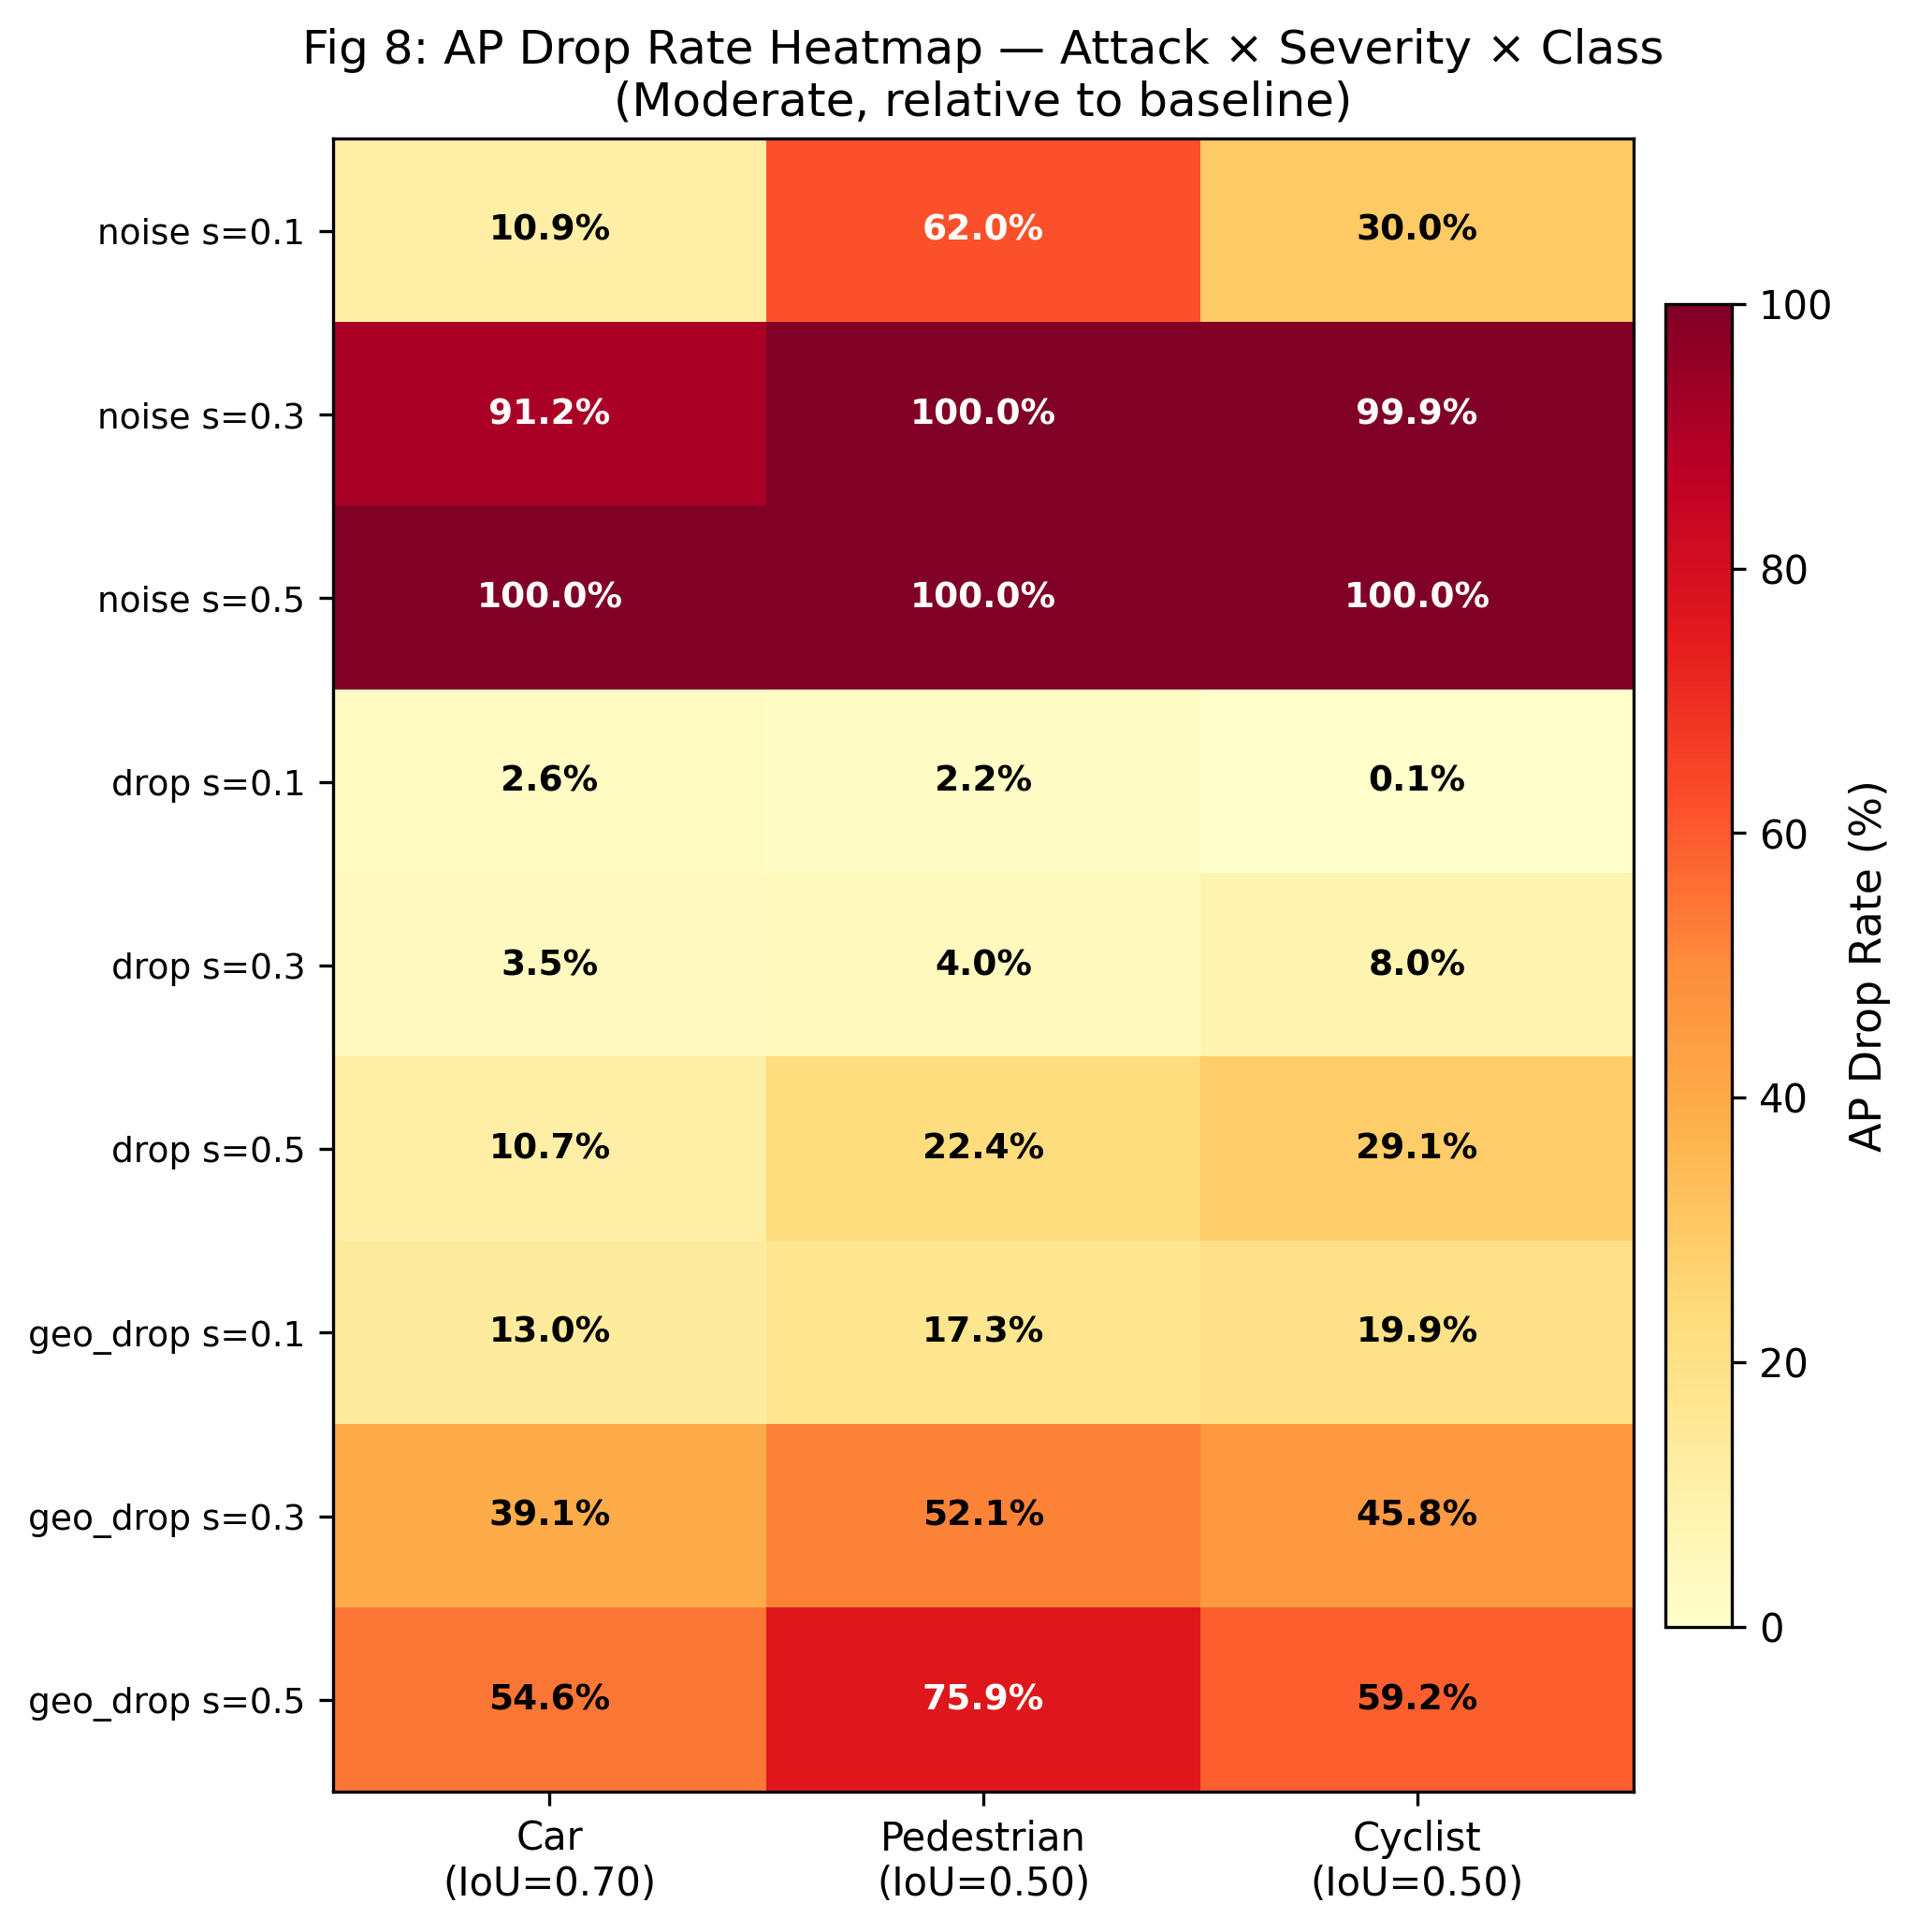
\includegraphics[width=0.75\linewidth]{fig8_map_heatmap.png}
\caption{AP下降率热力图（Moderate难度，相对基线百分比）。颜色越深表示AP下降越大。}
\label{fig:heatmap}
\end{figure}

从热力图可以观察到：
\begin{itemize}
  \item Pedestrian类别在多数攻击下AP下降最大，说明行人检测对点云扰动最敏感（IoU阈值0.50，目标体积小，点云稀疏）；
  \item 噪声攻击对Pedestrian和Cyclist的破坏效率高于Car，因为小目标的点云数量本就稀少，噪声更容易破坏其几何结构；
  \item Geo-Drop在所有类别上均表现出稳定的攻击效果，不像噪声攻击存在类别差异。
\end{itemize}

\subsection{难度等级分析}

图~\ref{fig:difficulty}对比了三种攻击在Easy、Moderate、Hard三个难度等级下的表现。

\begin{figure}[H]
\centering
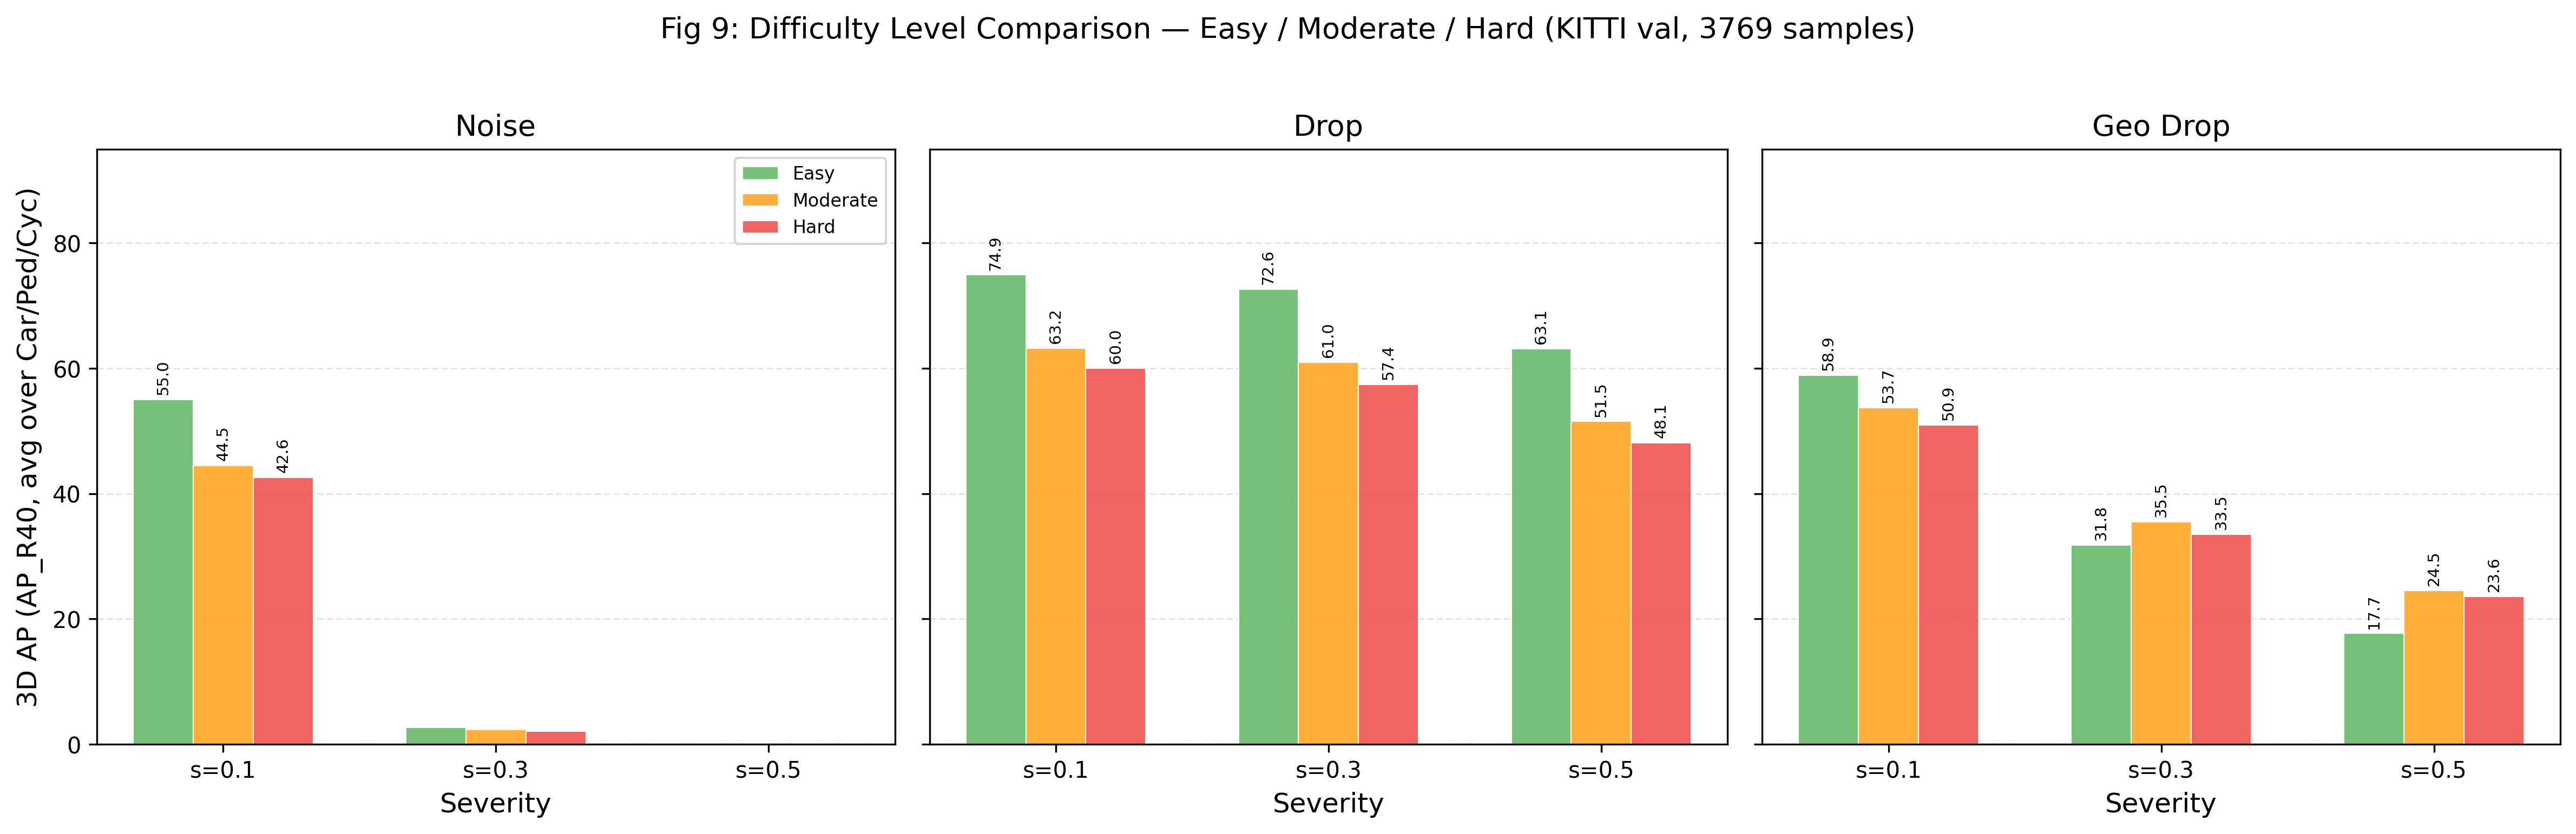
\includegraphics[width=0.95\linewidth]{fig9_difficulty_comparison.png}
\caption{难度等级对比：Easy/Moderate/Hard三个级别在三类黑盒攻击下的AP变化。}
\label{fig:difficulty}
\end{figure}

总体趋势为Easy $>$ Moderate $>$ Hard，这与基线性能的排序一致。值得注意的是，在噪声攻击下三个难度等级的AP几乎同步崩溃，说明噪声对点云的破坏是全局性的，不受目标遮挡程度和截断比例的调节。

\subsection{全部攻击方法总览}

图~\ref{fig:all_attacks}汇总了全部10种攻击方法在Moderate难度下的AP对比。

\begin{figure}[H]
\centering
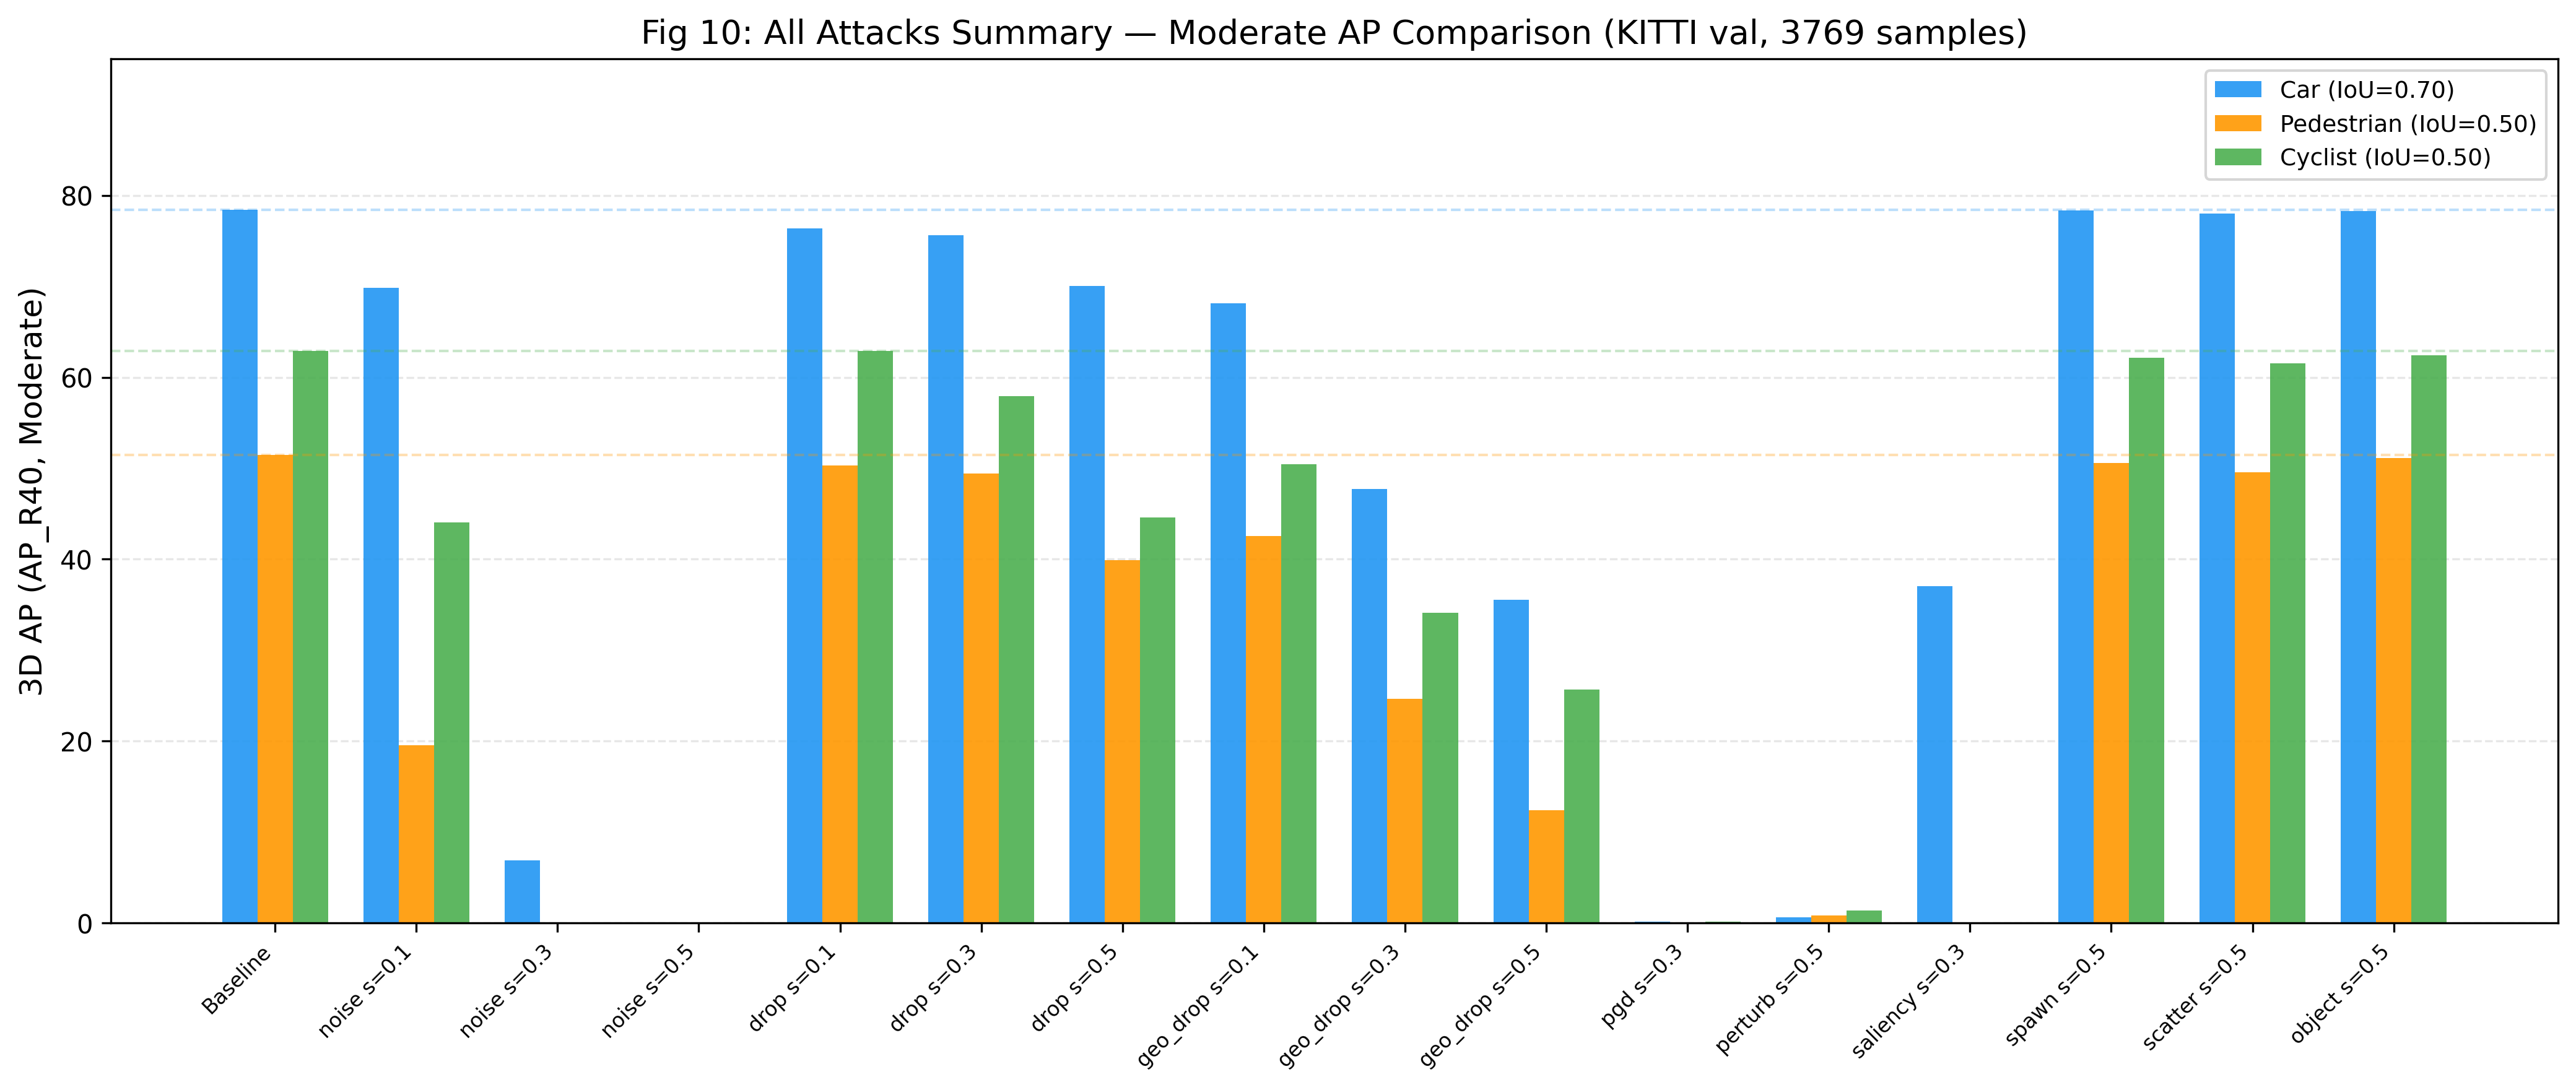
\includegraphics[width=0.95\linewidth]{fig10_all_attacks_summary.png}
\caption{全部攻击方法总览：10种攻击在Moderate难度下的3D AP对比。}
\label{fig:all_attacks}
\end{figure}

% ============================================================
% 5 讨论
% ============================================================
\section{讨论}

\subsection{攻击有效性排名}

综合全部实验结果，攻击有效性排名如下（按Car AP Moderate下降幅度）：

\begin{enumerate}
  \item \textbf{白盒扰动（PGD/Perturb）}：AP降至接近零。梯度指导的定向扰动是最高效的攻击方式；
  \item \textbf{噪声攻击（Noise $s \geq 0.3$）}：AP降至接近零。无需梯度的简单高斯噪声即可造成严重破坏；
  \item \textbf{几何感知删除（Geo-Drop $s=0.5$）}：AP下降55\%。定向删除策略显著优于随机删除；
  \item \textbf{显著性掩码删除（Saliency Mask）}：Car AP下降53\%。梯度定位关键体素，但仅作用于体素级别；
  \item \textbf{随机删除（Drop $s=0.5$）}：AP仅下降11\%。点云冗余性使其对随机删除具有天然鲁棒性；
  \item \textbf{插入类攻击}：AP变化$< 1$\%。攻击机制与AP评价指标不匹配。
\end{enumerate}

\subsection{几何感知删除 vs 随机删除}

Geo-Drop相比Drop的优势源于其针对性删除策略。随机删除均匀地减少点云密度，目标的局部几何特征虽然弱化但仍可辨识。而Geo-Drop优先删除距质心最近的点——这些点通常位于目标表面高密度区域，对目标检测和形状识别贡献最大。实验表明，在severity=0.5时，Geo-Drop的Car AP下降率（55\%）是Drop（11\%）的5倍，验证了"攻击质量比攻击数量更重要"的结论。

\subsection{物理可行性讨论}

本文实现的攻击方法在物理可行性上存在差异：
\begin{itemize}
  \item \textbf{噪声和删除攻击}具有较好的物理对应——LiDAR传感器在雨雾天气中会产生测量噪声，传感器遮挡会导致点云缺失；
  \item \textbf{Geo-Drop}在物理上对应"从特定角度遮挡目标"的攻击策略；
  \item \textbf{白盒攻击}（PGD/Perturb）需要精确控制每个体素的坐标偏移，在物理世界中难以精确实现；
  \item \textbf{幽灵模板}可通过3D打印或投影仪在物理世界中复现。
\end{itemize}

\subsection{防御启示}

基于实验发现，我们提出以下防御方向：
\begin{enumerate}
  \item \textbf{统计离群点移除（SOR）}：对噪声注入的异常点进行k近邻距离检验，过滤离群点；
  \item \textbf{体素均值滤波}：利用体素化过程的天然平滑效应，对每个体素内的点取均值；
  \item \textbf{对抗训练}：将对抗样本混入训练数据，提升模型的鲁棒性。
\end{enumerate}

% ============================================================
% 6 结论
% ============================================================
\section{结论}

本文在OpenPCDet工业级框架上系统化实现了针对PointPillars三维点云目标检测的对抗攻击与安全性评估。通过设计双通道攻击注入架构，实现了6类10种攻击方法，并在KITTI验证集3769个样本上完成全量mAP评估。主要结论如下：

(1)~PointPillars对坐标噪声攻击极为脆弱，severity $\geq 0.3$m的高斯噪声即可导致检测器完全失效；

(2)~提出的几何感知删除攻击（Geo-Drop）效果显著优于随机删除，证明定向攻击策略的有效性；

(3)~白盒梯度攻击（PGD/Perturb）效率最高，但需要模型梯度，实际应用场景受限；

(4)~插入类攻击对AP指标影响极小，提示评估体系需纳入假阳性率等补充指标。

未来工作将聚焦于：(a)~实现统计离群点移除等轻量级防御策略，并完成攻防闭环实验；(b)~探索基于代理模型的迁移攻击，评估对抗样本的跨架构迁移性；(c)~引入物理约束（如LiDAR射线方向约束），使攻击方法更具物理可实现性。

% ============================================================
% 参考文献
% ============================================================
\bibliographystyle{plainnat}
\bibliography{references}

\end{document}
